\documentclass{../Vorlage/mat}
\lstset{
	basicstyle=\small
}

\begin{document}
\maketitle{Sebastian Bliefert}{}{Nils Drebing}{}{Pascal Pieper}{}{11.01.2017}{3} \\

\section*{Aufgabe 1}
\subsection*{a)}
\lstset{language=python}
Die Implementierung des $A^{\star}$-Algorithmus erfolgt in der \textit{behaviour.py} . Das Ziel ist veränderbar, wenn die \textit{goal}-Variable über der Implementierung angepasst wird (standartmäßig auf 4.0, 4.0).\\
Um das Datenmanagement zu vereinfachen, wurde eine Klasse \textit{Node} entworfen. Diese speichert die benötigten Werte wie kürzeste Distanz, heuristische Bewertung für die Auswahl, Koordinaten und eine Referenz auf den Vorgänger. Die heuristische Bewertung ergibt sich dabei aus der aktuell kürzesten Distanz zu diesem Knoten + Distanz mittels euklidischer Norm zum Ziel.

\begin{lstlisting}
#datastucture used for handling coordinates and predecessors of wapoints
class Node:
    comingFrom = None   #reference to predecessor
    sDistance = 10000000.    #shortest path from start to goal
    gDistance = 10000000.    #heuristical score.
    coords = [0.,0.]
    neighbours = []     #neighbour nodes

    def __init__(self, coords):
        self.coords = coords
        self.comingFrom = self

    def __eq__(self, other):
        if isinstance(other, Node):
            return self.coords == other.coords
        else:
            return NotImplemented
\end{lstlisting}

Die Knoten werdne einmalig initialisiert. Das heißt zum einen, dass entsprechende Knoten zu allen Wegpunkten erstellt werden. Darüber hinaus werden die Nachbarknoten einmalig berechnet und in den Knoten gespeichert, um diese nicht bei jeder Iteration des $A^{\star}$ zu berechnen. Dabei sind mögliche Nachbarn all jene Wegpunkte, die direkt sichtbar und somit nicht durch eine Wand versperrt werden.

\begin{lstlisting}
#calculate neighbours of a given node
def calcNeighbourNodes(node):
    global nodes
    neighbours = []
    for n in nodes:
        if(not np.array_equal(n.coords, node.coords) 
        and checkIntersect(n.coords, node.coords)):
            neighbours.append(n)
    return neighbours
\end{lstlisting}

Der eigentliche Algorithmus ist nach den Vorgaben der Tutoriumsfolien implementiert worden. Die Dokumentation der einzelnen Schritte geht aus den Kommentaren des Quellcodes hervor.

\begin{lstlisting}
def aStar(pos):
    global nodes, goal
    path = []
    pos2d = [pos[0], pos[1]]
    openList = []
    closedList = []
    #add startnode, given by robotposition
    start = Node(pos2d)
    start.comingFrom = None
    start.sDistance = 0
    start.hDistance = dist(start.coords, goal)
    start.neighbours = calcNeighbourNodes(start)
    openList.append(start)

    while openList:
        #find node with lowest heuristic score
        current = min(openList, key=lambda x: x.hDistance)
        if current.coords == goal:
            #print "FOUND PATH"
            path = constructPath(current)
            return path
        #remove from openList since it is going to be expanded now
        openList.remove(current)
        closedList.append(current)

        #EXPANSION of current node
        for n in current.neighbours:
            #successor already checked, continue
            if n in closedList:
                continue
            #calculate distance travelled on this path
            tempDist = current.sDistance + dist(current.coords, n.coords)

            #add neighbour to openList
            if n not in openList:
                openList.append(n)
            #dont update distance if path is longer than the one before
            elif tempDist >= n.sDistance:
                continue

            # update neighbour's data
            n.comingFrom = current
            n.sDistance = tempDist
            n.hDistance = n.sDistance + dist(n.coords, goal)


    #failed, so returning an empty path
    return path
\end{lstlisting}

Die Rekonstruktion des Pfades erfolgt durch die rekursive Ausgabe der Koordinaten der jeweiligen Vorgängerknoten, bis kein Vorgänger bekannt ist.

\begin{lstlisting}
#reconstruct from goalnode
def constructPath(node):
    i = node
    path = []
    path.append(np.array(i.coords))
    while i.comingFrom != None:
        path.append(np.array(i.comingFrom.coords))
        i = i.comingFrom
    path.append(np.array(i.coords))
    #needed in reverse
    result = path[::-1]
    return result
\end{lstlisting}
\newpage
\subsection*{b)}
\begin{figure}[!htbp]
\centering
\begin{minipage}{.5\textwidth}
  \centering
  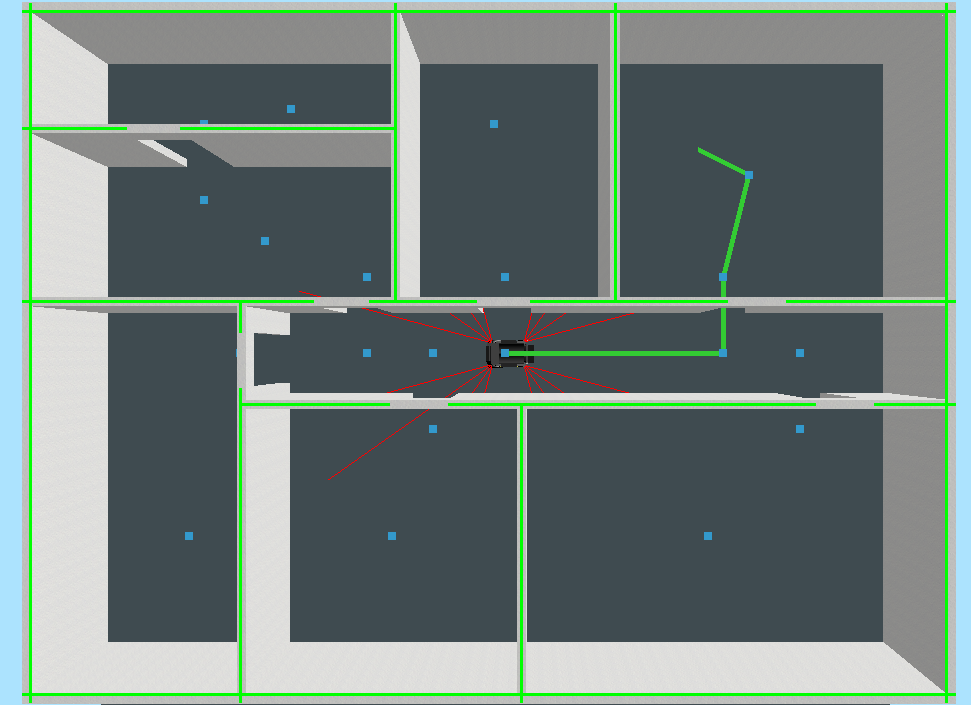
\includegraphics[scale=0.2]{astar_start.png}
  \captionof{figure}{$A^{\star}$ angewendet von der Startposition}
  \label{fig1}
\end{minipage}%%
\begin{minipage}{.5\textwidth}
  \centering
  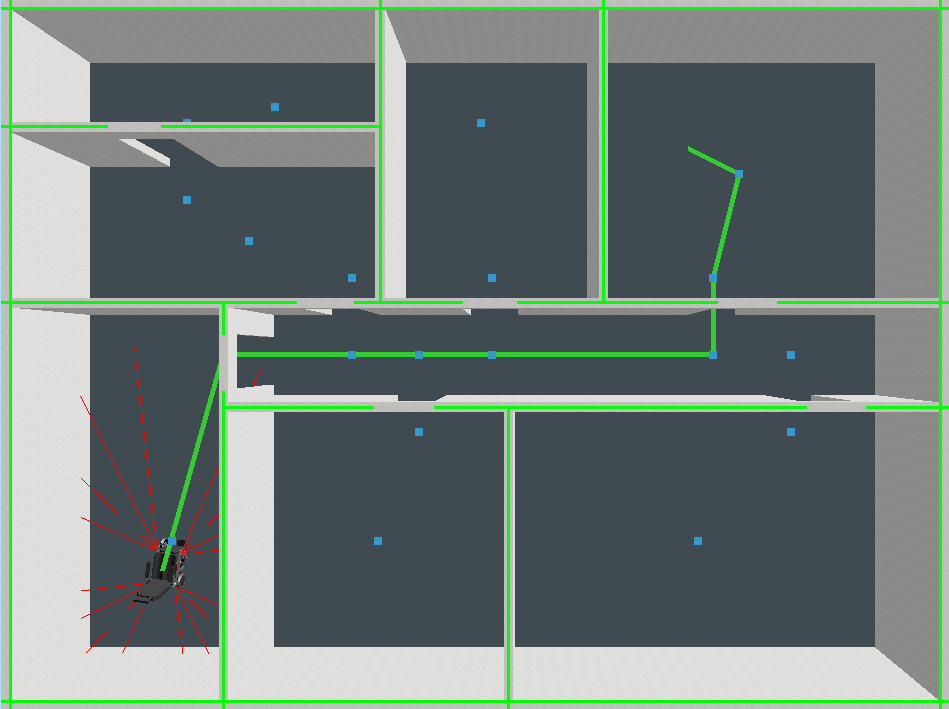
\includegraphics[scale=0.21]{astar_downleft.png}
  \captionof{figure}{$A^{\star}$ angewendet im Raum im Südwesten}
  \label{fig2}
\end{minipage}
\centering
\begin{minipage}{.5\textwidth}
  \centering
  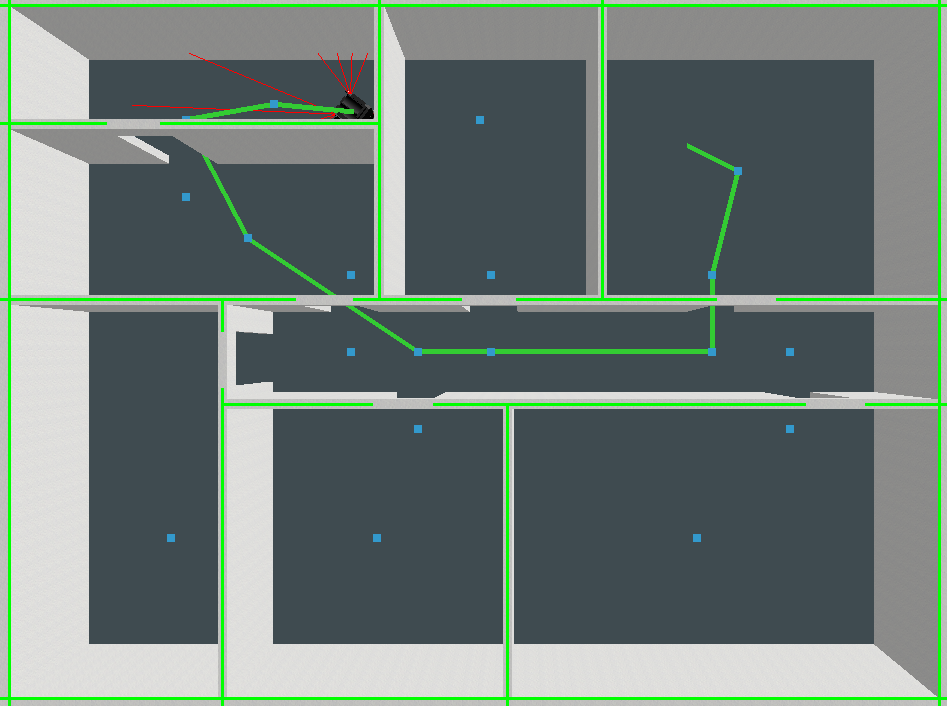
\includegraphics[scale=0.2]{astar_topleft.png}
  \captionof{figure}{$A^{\star}$ angewendet im Raum im Nordwesten}
  \label{fig3}
\end{minipage}%%
\begin{minipage}{.5\textwidth}
  \centering
  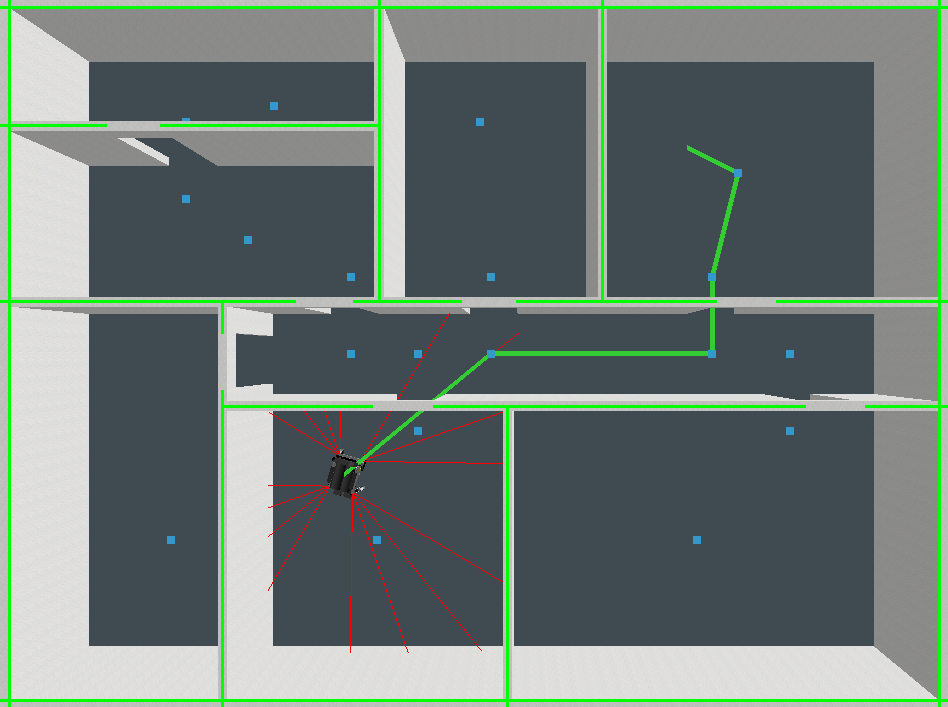
\includegraphics[scale=0.21]{astar_downmiddle.png}
  \captionof{figure}{$A^{\star}$ angewendet im Raum im Süden}
  \label{fig4}
\end{minipage}
\end{figure}

In den  Abbildungen \ref{fig3} und \ref{fig4} ist eine Problematik zu erkennen, die bei der Verwendung eines Braitenbergvehikels auftreten können: während die Bewegung auf Flächen ohne Hindernissen gut funktionieren würde, gäbe es erst Probleme beim Durchqueren der Türen. Hier wird nicht mit der Dimension des Roboters in der realen Welt gerechnet, sodass es gegen den Türrahmen fahren würde.
\newpage

\section*{Aufgabe 2}
\subsection*{Definiert Aktionen:}
\textbf{\_Essen(Rolf, Gericht)\_}\\
Preconditions: At(Rollstuhl, Esszimmer) $\wedge$ At(Gericht, Esszimer) $\wedge$ Nahrung(Gericht) $\wedge$ (Hungrig(Rolf) $\vee \neg$Hungrig(Rolf))\\
Postconditions: Satt(Rolf)


\textbf{\_Bewegen(Rollstuhl, Start, Ziel)\_}\\
Preconditions: Room(Start)$\wedge$Room(Ziel)$\wedge$At(Rollstuhl, Start) $\wedge$  Door(Start,open) $\wedge$ Door(Ziel,open)\\
Postconditions: At(Rollstuhl, Ziel)


\textbf{\_TürÖffnen(Tür)\_}\\
Preconditions: Door(Tür, closed)\\
Postconditions: Door(Tür, open)


\textbf{\_TürSchließen(Tür)\_}\\
Preconditions: Door(Tür, open)\\
Postconditions: Door(Tür, closed)


\textbf{\_Tragen(Dings, Start, Ziel)\_}\\
Preconditions: At(Rollstuhl, Dings) $\wedge$  Door(Start,open) $\wedge$ Door(Ziel,open)\\
Postconditions: At(Dings, Ziel), $\wedge$ At(Rollstuhl, Ziel)

\subsection*{Gebt Reihenfolgen an:}
%Init (Hungrig(Rolf) $\wedge$ at(Rollstuhl, Wohnzimmer) $\wedge$ At(Fertiggericht, Küche) $\wedge$ Door(Küche, closed) $\wedge$ Door(Wohnzimmer, closed) $\wedge$ Door(Esszimmer, closed) $\wedge$ Room(Küche) $\wedge$ Room(Esszimmer) $\wedge$ Room(Wohnzimmer) $\wedge$ Nahrung(Fertiggericht))

Init (Hungrig(Rolf) $\wedge$ at(Rollstuhl, Wohnzimmer) $\wedge$ At(Fertiggericht, Küche) $\wedge$ \underline{Door(Küche, closed)} $\wedge$ \underline{Door(Wohnzimmer, closed)} $\wedge$ \underline{Door(Esszimmer, closed)} $\wedge$ Room(Küche) $\wedge$ Room(Esszimmer) $\wedge$ Room(Wohnzimmer) $\wedge$ Nahrung(Fertiggericht))

TürÖffnen(Wohnzimmer), TürÖffnen(Küche), Türöffnen(Esszimmer)

(Hungrig(Rolf) $\wedge$ at(Rollstuhl, Wohnzimmer) $\wedge$ At(Fertiggericht, Küche) $\wedge$ \textit{\underline{Door(Küche, open)}} $\wedge$ \textit{\underline{Door(Wohnzimmer, open)}} $\wedge$ \textit{Door(Esszimmer, open)} $\wedge$ \underline{Room(Küche)} $\wedge$ Room(Esszimmer) $\wedge$ \underline{Room(Wohnzimmer)} $\wedge$ Nahrung(Fertiggericht))

Bewegen(Rollstuhl, Wohnzimmer, Küche)

(Hungrig(Rolf) $\wedge$ \underline{\textit{at(Rollstuhl, Küche)} $\wedge$ At(Fertiggericht, Küche)} $\wedge$ \underline{Door(Küche, open)} $\wedge$ Door(Wohnzimmer, open) $\wedge$ \underline{Door(Esszimmer, open)} $\wedge$ \underline{Room(Küche)} $\wedge$ \underline{Room(Esszimmer)} $\wedge$ Room(Wohnzimmer) $\wedge$ Nahrung(Fertiggericht))

Tragen(Fertiggericht, Küche, Esszimmer)

(Hungrig(Rolf) $\wedge$ \underline{\textit{at(Rollstuhl, Esszimmer) $\wedge$ At(Fertiggericht, Esszimmer)}} $\wedge$ Door(Küche, open) $\wedge$ Door(Wohnzimmer, open) $\wedge$ Door(Esszimmer, open) $\wedge$ Room(Küche) $\wedge$ Room(Esszimmer) $\wedge$ Room(Wohnzimmer) $\wedge$ Nahrung(Fertiggericht))

Essen(Fertiggericht)

(\textit{Satt(Rolf)} $\wedge$ \underline{at(Rollstuhl, Esszimmer)} $\wedge$ Door(Küche, open) $\wedge$ \underline{Door(Wohnzimmer, open)} $\wedge$ \underline{Door(Esszimmer, open)} $\wedge$ Room(Küche) $\wedge$ \underline{Room(Esszimmer)} $\wedge$ \underline{Room(Wohnzimmer)})

Bewegen(Rollstuhl, Wohnzimmer)

(Satt(Rolf) $\wedge$ \textit{at(Rollstuhl, Wohnzimmer)}$\wedge$ Door(Küche, open) $\wedge$ \underline{Door(Wohnzimmer, open)} $\wedge$ Door(Esszimmer, open) $\wedge$ Room(Küche) $\wedge$ Room(Esszimmer) $\wedge$ Room(Wohnzimmer))

TürSchließen(Wohnzimmer)

(Satt(Rolf) $\wedge$ at(Rollstuhl, Wohnzimmer) $\wedge$ Door(Küche, open) $\wedge$ \textit{Door(Wohnzimmer, closed)} $\wedge$ Door(Esszimmer, open) $\wedge$ Room(Küche) $\wedge$ Room(Esszimmer) $\wedge$ Room(Wohnzimmer))


\subsection*{A* for STRIPS}
\textbf{Expansion}\\
Auf Basis des aktuellen Zustandes wird geprüft, welche Aktionen ausgeführt werden können. Dann werden die möglichen Folgezustände ermittelt, indem die möglichen Aktionen auf den aktuellen Zustand angewendet werden. Für die Folgezustände, die nicht der closedList stehen, werden die Heuristik und die Kosten berechnet und dann die Zustände zur openList hinzugefügt. Zum Schluss wird der Basiszustand von der openList entfernt und zur closedList hinzugefügt.\\
\\
\textbf{Heuristik}\\
Sei:\\
$T = $ Menge der Teilzustände im Zielzustand\\
$F = $ Menge der Teilzustände im betrachteten Zustand\\
$S = T \bigcap F$\\
\\
Eine mögliche Heuristik wäre: $h(x) = \frac{|S|}{|T|}$\\
Dabei wäre die Heuristik zu maximieren.\\
\\
\textbf{Kosten}\\
Die Kosten für die Transition von einem Zustand in einen möglichen Folgezustand könnten an der dafür nötigen Aktion festgemacht werden. Hier könnte zum Beispiel die Anzahl der Effekte der Aktion als Kosten der Funktion festgelegt werden. Dabei wäre dann irrelevant, wie viele Einzelaktionen ausgeführt werden würden, sondern nur relevant, wie viele Effekte insgesamt auftreten würden. Um die Anzahl der ausgeführten Aktionen mit einzubeziehen, könnten die Kosten als Anzahl der Effekte einer Aktion plus eins festgelegt werden.\\
\\
\textbf{Kann man A* einsetzen um STRIPS Probleme zu lösen?}
Ja, dies ist mit dem oben gemachten Angaben möglich.
\end{document}
